\documentclass[a4paper,12pt]{article}
\usepackage[utf8]{inputenc}
\usepackage[T1]{fontenc}
\usepackage[magyar]{babel}
\usepackage{indentfirst}
\usepackage{amsmath}
\usepackage{graphicx}
\frenchspacing
\author{Belényesi Roland}

\begin{document}
\section{Bevezetés}
A big data napjainkban az egyik vezető címke az informatikai terminológiák körében, különböző címekkel ellátva, mint: 
\textsl{Sikerhez és boldogsághoz vezet a big data}~\cite{ori} vagy 
\textsl{Új korszak kezdődött a tudományban.}~\cite{oria} De mit is jelent pontosan? Nincs explicit kimondott meghatározás a fogalomra, de Doug Laney 2001-es definíciója egy jó kindulópontnak tekinthető: az adatok nagy mennyiségben (volume), gyorsan(velocity) és különböző formátumban(variety) jelennek meg (3V's)~\cite{3v}.Azonban, ma már kiegészíthetjük ezt a fogalmat még 2V-vel: bizonyosság(veracity) és érték(value).~\cite{5v} Az adatmennyiség amit előállítunk exponenciálisan növekszik olyan szintre, aminek tárolását, menedzselését és elemzését már nem tudjuk megoldani a saját, lokális erőforrásainkon belül az eddig megszokott adatelemzési eszközökkel, mint például Microsoft Excel, vagy különböző relációs adatbázis technológiák által.
Becslések~\cite{2020} szerint az adatok mennyisége kétévente duplázódik, így 2020-ra az összekézben forgó adatmennyiség elérheti a 44 zetabájtnyi (vagy 44 trillió gigabájtnyi) mennyiséget.
\linebreak

A "big data" lehetőséget biztosít arra, hogy ezeket az adatokat ne csak tároljuk, hanem új módokon tanuljunk belőle, értéket állítsunk elő, többet megtudjunk ügyfeleinkről, a saját üzleti folyamatainkról, ami versenyelőnyhöz vezethet. E mellett az áttörő kutatások számát is megnöveli azáltal, hogy rejtett összefüggéseket mutat meg.~\cite{brk} 

A cloud computing, és új technológiák megszületése és az, hogy a fizikai világ egyre jobban átterelődik az online térbe, új nehézségeket állít elő mind az adatokat kiszolgáló, mind az adatokat elemző infrastruktúrák számára. Ezek a problémák komoly gondot jelentek az informatikai iparnak, mivel érintik az fizikai manifesztációt (hardver), mind az ezt vezérlő és feldolgozó réteget (szoftver és algoritmus). Ezek a problémák,~\cite{dst} --amelyek a tradícionális adattárház technológiákra jellemzőek-- többek között származhatnak a hiba-tolerancia hiányából, a sokféle adatfajtából,a párhuzamosság hiányából, mely azt eredményezi, hogy a mai technológia fejlettség (és a központi számítási egységek fizikailag limitáltsága miatt) nem lesz megfelelő számítási teljesítmény a megnövekedett adatmennyiség menedzselésére.

\section{A dolgozat célja}

A technológia fejlődése és a számítási teljesítmény megnövekedése hozta létre azt az üzleti igényt~\cite{rta}, hogy egyre gyorsabban, egyre nagyobb adatmennyiség feldolgozása történjen meg. Ilyen igény például:csalás felderítés~\cite{fraud}, "dolgok" internete (IoT)~\cite{iot} vagy alkalmazás monitoring~\cite{ganalitycs}. Ez az adatfeldolgozási sebesség olyan szintre eljutott, hogy közel valós időben, az adat keletkezése után megtörténhet ennek feldolgozása. Ilyen gyorsaságú adatfeldolgozásra csak elosztott rendszerek segítségével vagyunk képesek,~\cite{ucl} amelyek felépítésükből fakadóan sok lehetőség és költség jellemez, amelyeket a későbbiekben fogok kifejteni. A dolgozatomban használt Apache Flink (mely az Apache Foundation egyik legújabb és legmodernebb terméke) platform közel 40 millió elem feldolgozására képes egy 40 magos architektúrán másodpercenként.~\cite{flink}.  \linebreak

Ahhoz, hogy ezt az adatmennyiséget ki tudjuk elemezni és ajánlásokat tudjunk adni, gépi tanulásra van szükségünk. A gépi tanulás az informatikának és a matematikának egy olyan ága, amely az adatok folyamatos betáplálása során új ismereteket szolgáltat, megpróbál előrejelzéseket adni anélkül, hogy explicit módon be lenne erre programozva. ~\cite{ml}. A választott metódus a stochastic gradient descent (SGD, sztochasztikus gradiens ajánlás)~\cite{sgd}, amely egy olyan egyszerűsítési illetve optimalizációs eljárás, ahol adott célfüggvény gradiensét folyamatosan, iteratív módon számoljuk ki. Célom az, hogy megtervezzem Apache Flink alatt az SGD algoritmust, összehasonlítsam a teljesítményét a már implementált algoritmusokkal és megkezdjem a szükséges módosítások implementálást.

\section{Gépi tanulás}

Amikor tanulunk, a célünk, hogy minél jobb eredményeket érjünk el a számonkérésen, vagy minél több tudást halmozzunk fel, amit a későbbiek során (valószínűsíthetően) hasznosítani tudunk. A gépi tanulásnak is ugyanez a célja, különböző modellek megalkotása után a megadott példákból (input adat) különböző kimeneteket (output adat) ad ki. Az input adatokból próbál általánosítani oly módon, hogy az felhasználható legyen számára ismeretlen problémák során. Gépi tanulást használunk például: 
\begin{itemize}
\item web keresés
\item spam szűrés
\item ajánló rendszerek
\item online hírdetések
\end{itemize}
esetén is. 
Egy 2011-es Mckinsey riport ~\cite{mckinsey} szerint a gépi tanulás (illetve a prediktív analitika) lesz a következő évek innovációinak alapja. IBM Watson-ja~\cite{watson}, már képes a beadott tünetek alapján, megjósolni, hogy mi lehet a páciens betegsége (egyelőre még csak fejlesztőknek API-n keresztül). \linebreak

Általánosan fogalmazva, az adat amit betáplálunk a gépi tanulás modellünkbe, tréning példáknak (training set) nevezzük. A tréning példák $x$, $y$ párokat tartalmaznak, ahol $x$ az érték vektor (feature vector). Minden $x$ érték: kategórikus (diszkrét értékeksorozatból származik, pl{kék, piros, sárga}) vagy numerikus (az érték egész vagy valós szám). $y$ a címke (label), ami kategorizáló érték $x$-re nézve.A célünk az, hogy felfedezzük azt az 
\begin{equation*} y=f(x)
\end{equation*}
függvényt, ahol a legjobban előre tudjuk jelezni az $y$ értéket a meghatározott $x$-re nézve.

Két fő csoportja van a gépi tanulási algoritmusoknak: a felügyelt (supervised) és nem felügyelt (unsupervised) tanítás.

\section{Felügyelt tanítás}
Fontos, hogy szétválasszuk az adatainkat tréning és teszt adatokra. Ez biztosítja azt, hogy ne fordulhasson elő az a probléma, hogy a modellünk túlságosan fontos súllyal vesz egyes objektumokat az adatsoron (amik nem jellemzőek a lehetséges valós adatokra), ami azt eredményezi, hogy a valós problémákon már nem fog eredményesen működni. A problémát túltanulásnak vagy magolásnak (overfitting) nevezik.


\begin{figure}[ht!]
\centering
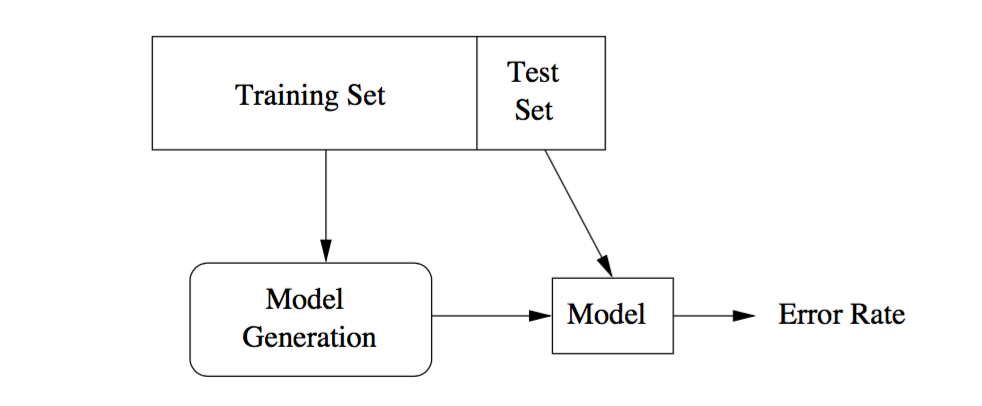
\includegraphics[width=90mm]{img/ml.png}
\caption{Gépi tanulás általános modellje \label{overflow}}
\end{figure}

\section{Nem felügyelt tanítás}
Nem felügyelt tanítás esetén adottak: $(x_1, x_2, ..., x_n)$ adataink, és nincs célfüggvényünk, vagy elvárt kimenetünk. Alapvetően nem struktúrált \textsl{zajból} próbálunk mintázatot keresni, olyan modellt létrehozni, ami jól reprezentálja adatok valószínűségi eloszlálást. Annak ellenére, hogy nincs információnk arról, hogy az egyes adatok milyen kapcsolatban vannak egymással, $(x_t)$ valószínűségi eloszlását meg tudjuk jósolni  $(x_1,x_2, ..., x_{t-1})$ alapján, ahol  $P(x_t|x_1,x_2, ..., x_{t-1})$
Egyszerűbb esetekben, ahol az input sorrend irreleváns, lehet modellt építeni az adatra, ahol$(x_1, x_2, ...)$ az adatsorunk, és ezek függetlenül de identically származnak a $P(x)^2$

\section{Ajánlórendszerek}

\section{Batch}
\section{Lambda-architektúra}
\section{Streaming}
bounded, unbounded
\section{Time-agonistic}
\begin{itemize}
\item Event time
\item Proccesing time
\end{itemize}
\section{Flink(Spark/Storm/Mapreduce)}
\section{Ajánlórendszerek}
\begin{itemize}
\item Collaborative filtering
\item Content based
\end{itemize}
\section{ALS}
\section{DSG}
\section{Java, Scala}
Max 1 oldal, miért ez lett
\section{Dcg,nDCG}


\end{document}

\begin{thebibliography}{99}
\bibitem{ori}http://www.origo.hu/techbazis/20151020-big-data-adatok-elemzes-siker-ceg-startup.html
\bibitem{oria}http://www.origo.hu/tudomany/20131014-big-data-adatelemzes-tudomany-adatbanyaszat-informatika.html
\bibitem{3v}http://blogs.gartner.com/doug-laney/files/2012/01/ad949-3D-Data-Management-Controlling-Data-Volume-Velocity-and-Variety.pdf
\bibitem{5v}http://enterprisearchitects.com/the-5v-s-of-big-data/
\bibitem{log}http://www.infoworld.com/article/2608064/big-data/big-data-log-analysis-thrives-on-machine-learning.html
\bibitem{brk}http://www.informationweek.com/government/big-data-analytics/big-data-disease-breakthroughs/d/d-id/1316310
\bibitem{2020}http://www.emc.com/leadership/digital-universe/2014iview/executive-summary.htm
\bibitem{sas}http://www.sas.com/en_us/insights/articles/big-data/big-data-and-iot-two-sides-of-the-same-coin.html
\bibitem{dst}http://www.bogotobogo.com/WebTechnologies/distributedcomputing.php
\bibitem{rta}https://en.wikipedia.org/wiki/Real-time_business_intelligence
\bibitem{fraud}http://www.pactera.com/resources/blog/how-big-data-is-revolutionizing-fraud-detection-in-financial-services/
\bibitem{iot}https://datafloq.com/read/real-time-analytics-internet-of-things/943
\bibitem{ganalitycs}https://support.google.com/analytics/answer/1638635?hl=en
\bibitem{ucl}http://www0.cs.ucl.ac.uk/staff/ucacwxe/lectures/ds98-99/dsee3.pdf
\bibitem{flink}http://flink.apache.org/features.html#unified-stream-amp-batch-processing
\bibitem{ml}http://www.sas.com/en_us/insights/analytics/machine-learning.html
\bibitem{sgd}http://research.microsoft.com/pubs/192769/tricks-2012.pdf
\bibitem{mckinsey}http://www.mckinsey.com/insights/business_technology/big_data_the_next_frontier_for_innovation
\bibitem{watson}http://www-03.ibm.com/innovation/us/engines/assets/9442_Watson_A_System_White_Paper_POW03061-USEN-00_Final_Feb10_11.pdf
\end{thebibliography}